\documentclass{article}
\usepackage[utf8]{inputenc}
\usepackage{graphicx}
\usepackage{tikz}

\title{How long should one stare at the Haar-Ginibre railway?}
\author{Carlos Vargas}
\date{\today}

\begin{document}
	\maketitle	
	\begin{abstract}
		We study the eigenvalues of a family of matrices 
		$$R(s,t) = \alpha(s)C + \beta(s)U(t),$$ 
		periodic on the parameter $t\in [0,1]$, with $s\in [0, 1]$,   
		determined by a realization of a Ginibre matrix $C$ 
		and a rotating unitary matrix $U(t)$. 
		
		The matrices in this family are approximations of 
		R-diagonal elements in free probability, studied by 
		Haagerup-Larsen [?], Kemp-Speicher [?] and P. Zhong [?]. 
		
		We study the eigenvalue collisions for all values of $s$ and $t$. 
		To do this, we fix $s$, and increase the periodic value $t$, 
		while keeping track of each eigenvalue.	
		
		Unless $s$ is too close to $0$ or $1$, 
		the process leads in general to a non-tivial permutation $\sigma(s)$, 
		with pleasing visualizations of flowing, repellent eigenvalues.
		
		The intricate web of paths that the eigenvalues collectively traverse 
		remains quite stable for small variations in $s$. 
		However, the actual permutation $\sigma(s + \Delta s)$ 
		itself does present variations, 
		indicating eigenvalue collisions 
		at some intermediate values $(s,t)$, $s\in (s, s + \Delta s)$,
		which explain the permutation discrepancy. 
		
		The eigenvalue 'track-flips' that occur before/after these colissions 
		are the essential differences between consecutive railway systems, 
		as the eigenvalues proceed to team-up to whirl around themselves and then around zero.
		
		We report some first statistics about these processes and their collisions, 
		and we include a simple package to perform/store/display these (parallellizable) 
		computations and visualizations.
 	\end{abstract}
	\section{Introduction}

	Let $C$ be a realization of an $N\times N$ Ginibre matrix and, for $t\in [0,1]$ and 
	let $\omega$ is the first clock-wise non-trivial complex $N$-th root of $1$. Let
	$$U(t) = \mathrm{diag}(\omega^{tN}, \omega^{tN+1}, \omega^{tN+2}, \dots   , \omega^{tN+N-1}),$$ 
	be a diagonal matrix with equi-distant points along the circle. Notice that $U(0) = U(1)$.

	We want to study the eigenvalues of the matrix model:
	$$R(s,t) = \alpha(s)C + \beta(s)U(t),\quad  \alpha(s)= \cos((s\pi)/2), \beta(s)= \sin((s\pi) /2)U(t),$$ 
	which is periodic on $t\in [0,1]$ for fixed $s$.

	In general it is quite a task to compute distributions 
	of non-selfadjoint random matrix models. 
	The family of matrices in this model, however, are approximations of R-diagonal elements in free probability, 
	for which some actual computations are possible [?,?]. 

	Depending on the values of $\alpha$ and $\beta$, 
	the asymptotic distributions are supported on a centered annulus or disk,  
	(see Figure). 

	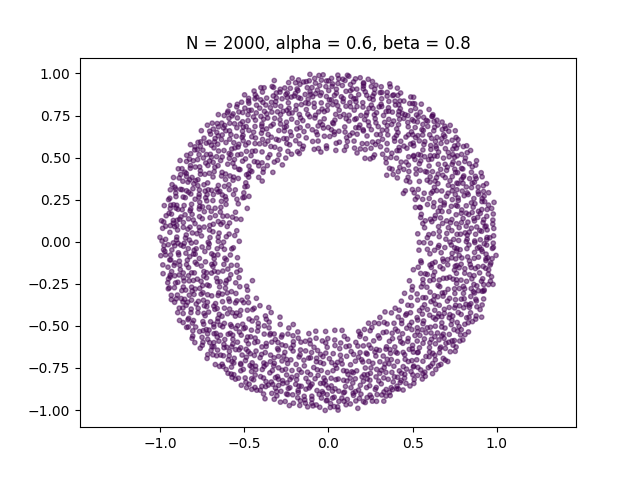
\includegraphics[width=0.5\textwidth]{/home/charli/Math/eigenvalueTracking/animatedGinibre/Figure_1.png}
	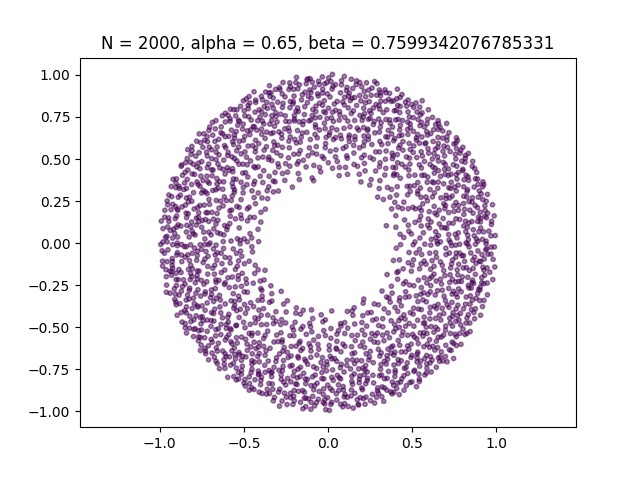
\includegraphics[width=0.5\textwidth]{/home/charli/Math/eigenvalueTracking/animatedGinibre/Figure_3.png}
	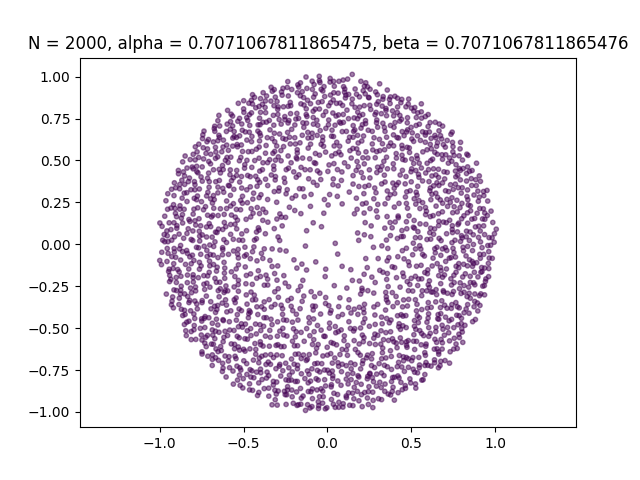
\includegraphics[width=0.5\textwidth]{/home/charli/Math/eigenvalueTracking/animatedGinibre/Figure_2.png}

	We choose $\alpha(s) = \cos(s \pi /2)$ and $\beta(s) = \sin(s \pi /2)$ 
	specificaly to make the outer radious of the model equal to one. 
	The eigenvalues for any other positive pairs $(\alpha, \beta)$ can be obtained 
	by scaling values within our parametrization.
	
	In this work we mainly want to draw attention to the effect of increasing $t$,
	which 'turns' the eigenvalues of the model clockwise.

	In the figure, we show the eigenvalues (red circles) tracking the eigenvalues 
	at after small increases of t (blue stars)
	
	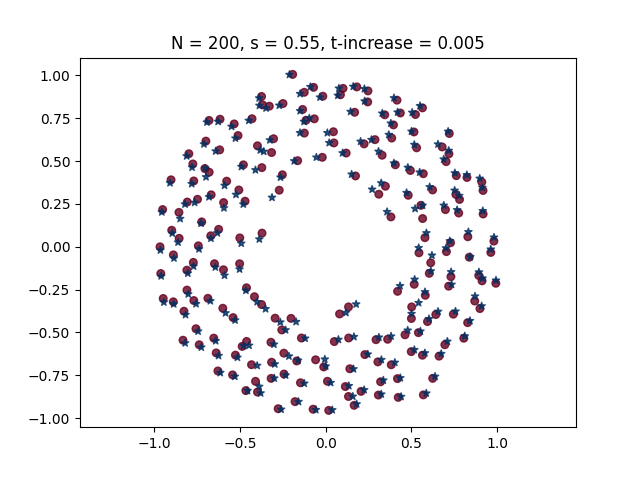
\includegraphics[width=0.5\textwidth]{/home/charli/Math/eigenvalueTracking/animatedGinibre/Figure_10.png} 
	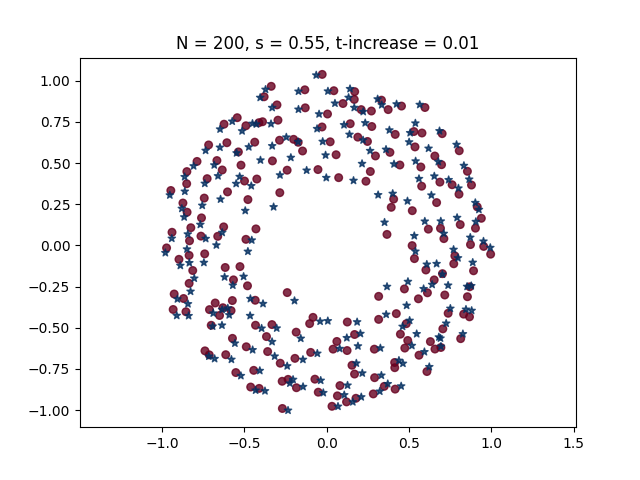
\includegraphics[width=0.5\textwidth]{/home/charli/Math/eigenvalueTracking/animatedGinibre/Figure_8.png} 
	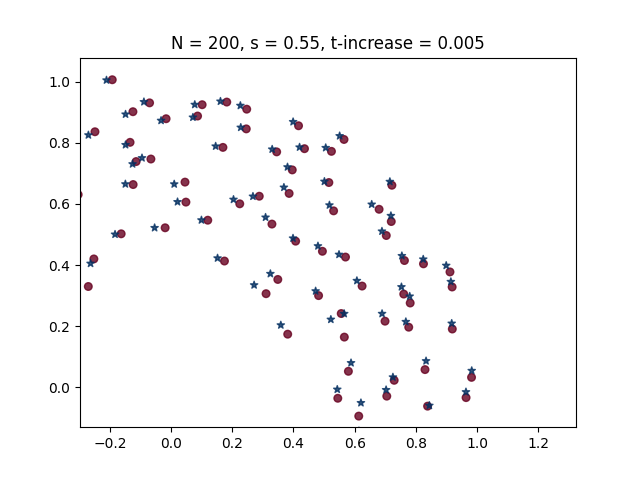
\includegraphics[width=0.5\textwidth]{/home/charli/Math/eigenvalueTracking/animatedGinibre/Figure_11.png} 
	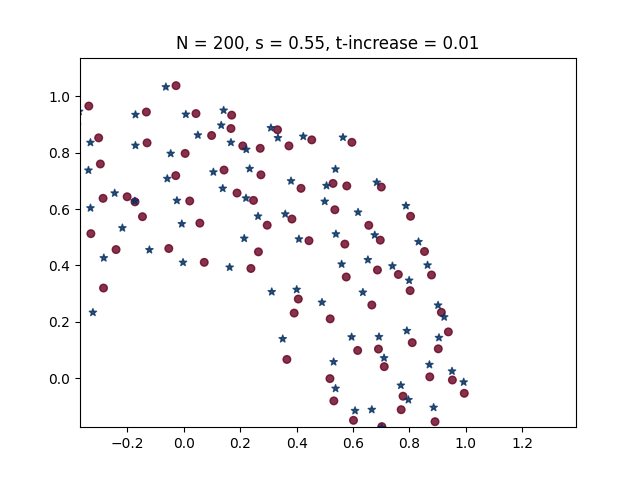
\includegraphics[width=0.5\textwidth]{/home/charli/Math/eigenvalueTracking/animatedGinibre/Figure_9.png}
	
	\newpage
	\section{Permutation $\sigma(s)$}

	Unless $s$ is too close to $0$ or $1$, the process of increasing the periodic parameter $t$
	leads in general to a non-trivial permutation $\sigma(s)$ after reaching $t=1$.
	Indeed, since eigenvalues at the outer part of the annulus are moving more slowly, 
	they wont be able to perform a complete turn, 
	thus falling into some other eigenvalue's original position at $t=0$.

	Let us consider first the eigenvalues of $R(0,t) = R(0,0)$. 
	These are just the eigenvalues of a complex Gaussian Ginibre matrix $C$,
	with explicit joint distribution 
	$$(insert formula)$$

	As $N\to \infty$ this distribution converges to uniform distribution on the unit disc.

	To be able to store the relevant data properly, 
	we will first label the eigenvalues increasingly by norm at $R(0,0)$. 
	
	Then we consider all the values $R(s,0)$, 
	(with $t = 0$) and increase $s$ slowly, keeping track of the labels continuosly 
	until we reach $R(1,0)$. 
	
	In case of ambiguity of eigenvalue tracking, a refinement is performent on 
	the partition on $s \in [0,1]$.

	After this is performed and a continous ordering of the eigenvalues for all values 
	of $s$ and $t=0$ has been achieved, now we consider, for each $s\in [0,1]$ 
	(in the $s$-partition) the process $R(s,t)$ when increasing $t$ from $0$ to $1$, 
	keeping track of the eigenvalues.

	For some $s$ relatively small we may observe some differences on the permutations, 
	while noticing very little discrepancies on the collective trails traveled.

	In the Figure $s=0.0500, 0.0505, 0.0510, 0.0515$. 
	The eigenvalue tracks are colored according to cycle length 
	
	(yellow = singletons, orange = 2-cycles, ... , darker cycles of greater length). 
	
	Notice first the large, $26$-element purple cycle $[1, 7, 19, 51, 25, \dots, 16, 8]$. 

	The collective paths remain almost unaltered, 
	but there are some few eigenvalue collisions in between each frame:
	
	\begin{figure}[ht]
		\centering
		\begin{minipage}{0.48\textwidth}
			\centering
			\includegraphics[width=\textwidth]{/home/charli/Math/eigenvalueTracking/animatedGinibre/N100S00500.png}
		\end{minipage}
		\hfill
		\begin{minipage}{0.48\textwidth}
			\centering
			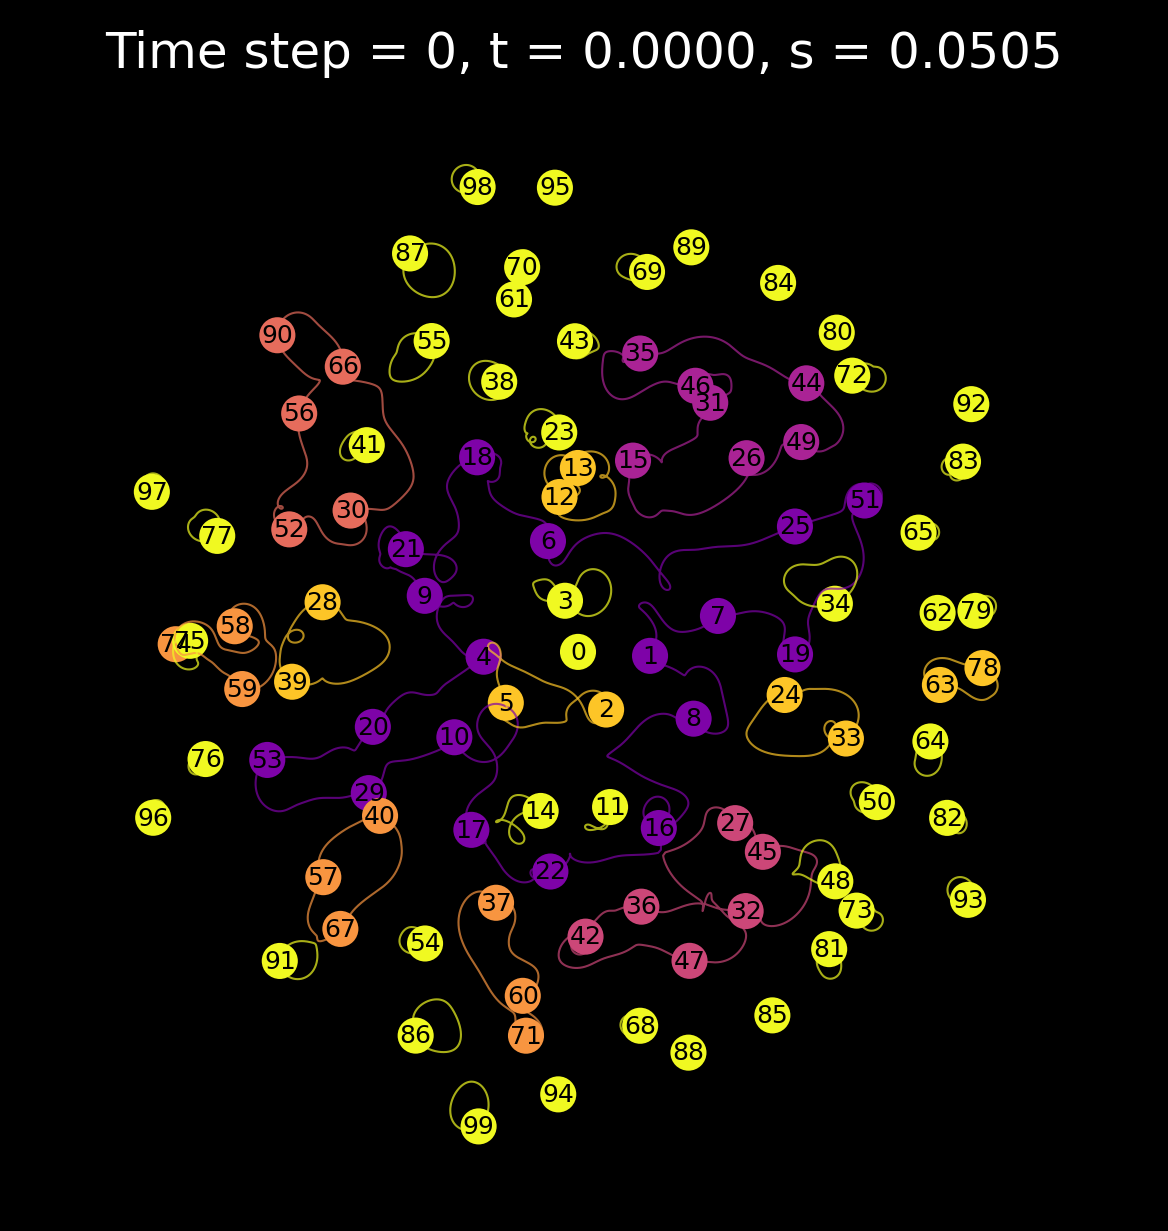
\includegraphics[width=\textwidth]{/home/charli/Math/eigenvalueTracking/animatedGinibre/N100s00505.png}
		\end{minipage}
		\vspace{0.5em}
		\begin{minipage}{0.48\textwidth}
			\centering
			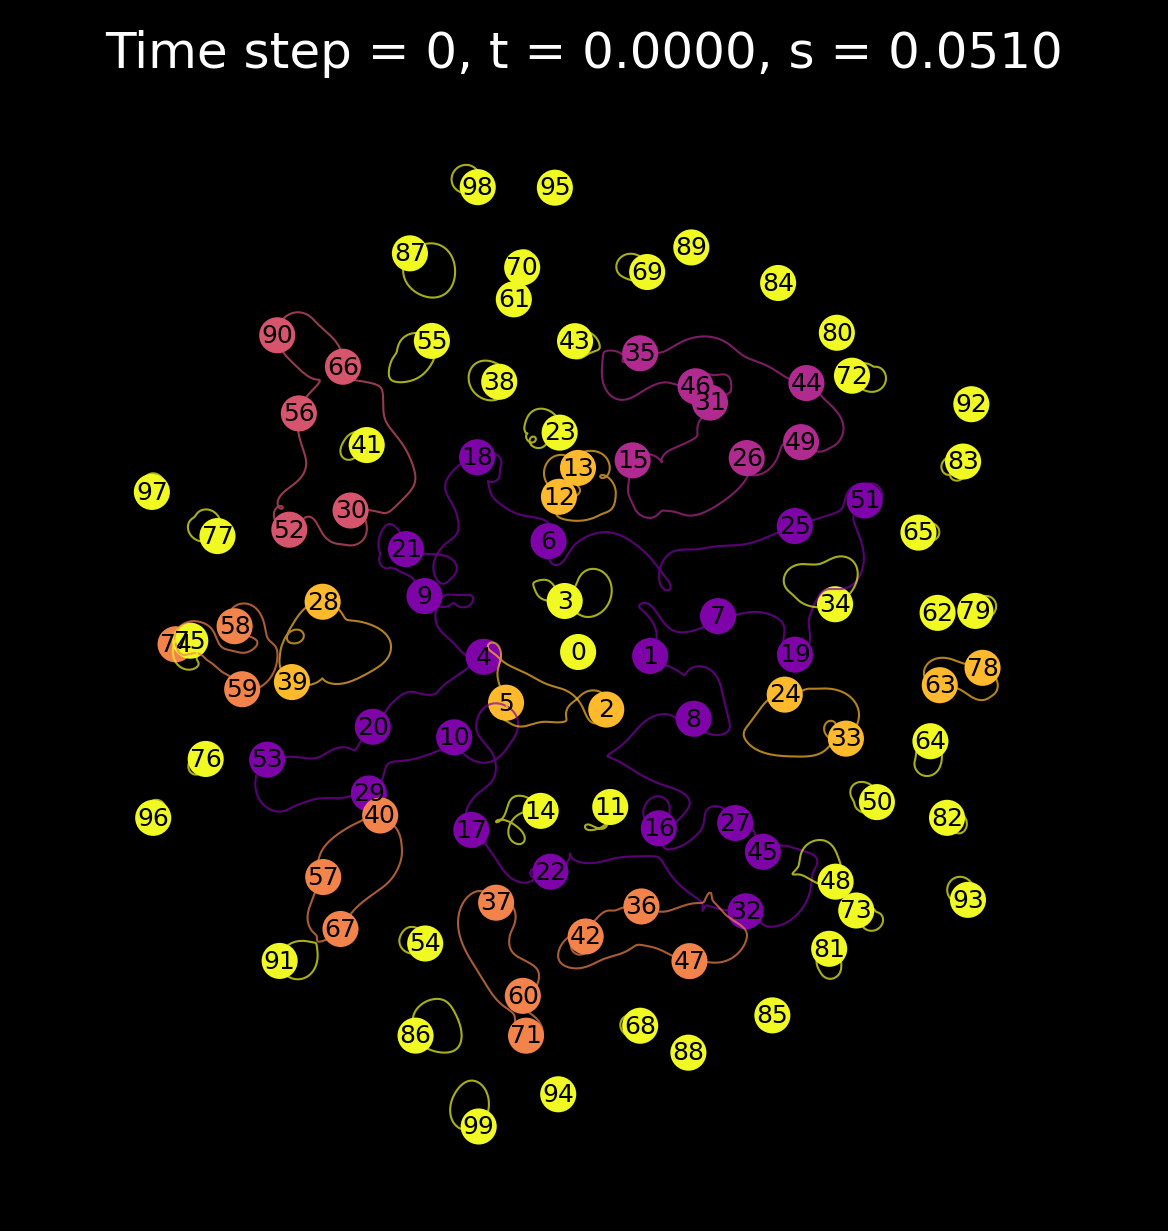
\includegraphics[width=\textwidth]{/home/charli/Math/eigenvalueTracking/animatedGinibre/N100s00510.png}
		\end{minipage}
		\hfill
		\begin{minipage}{0.48\textwidth}
			\centering
			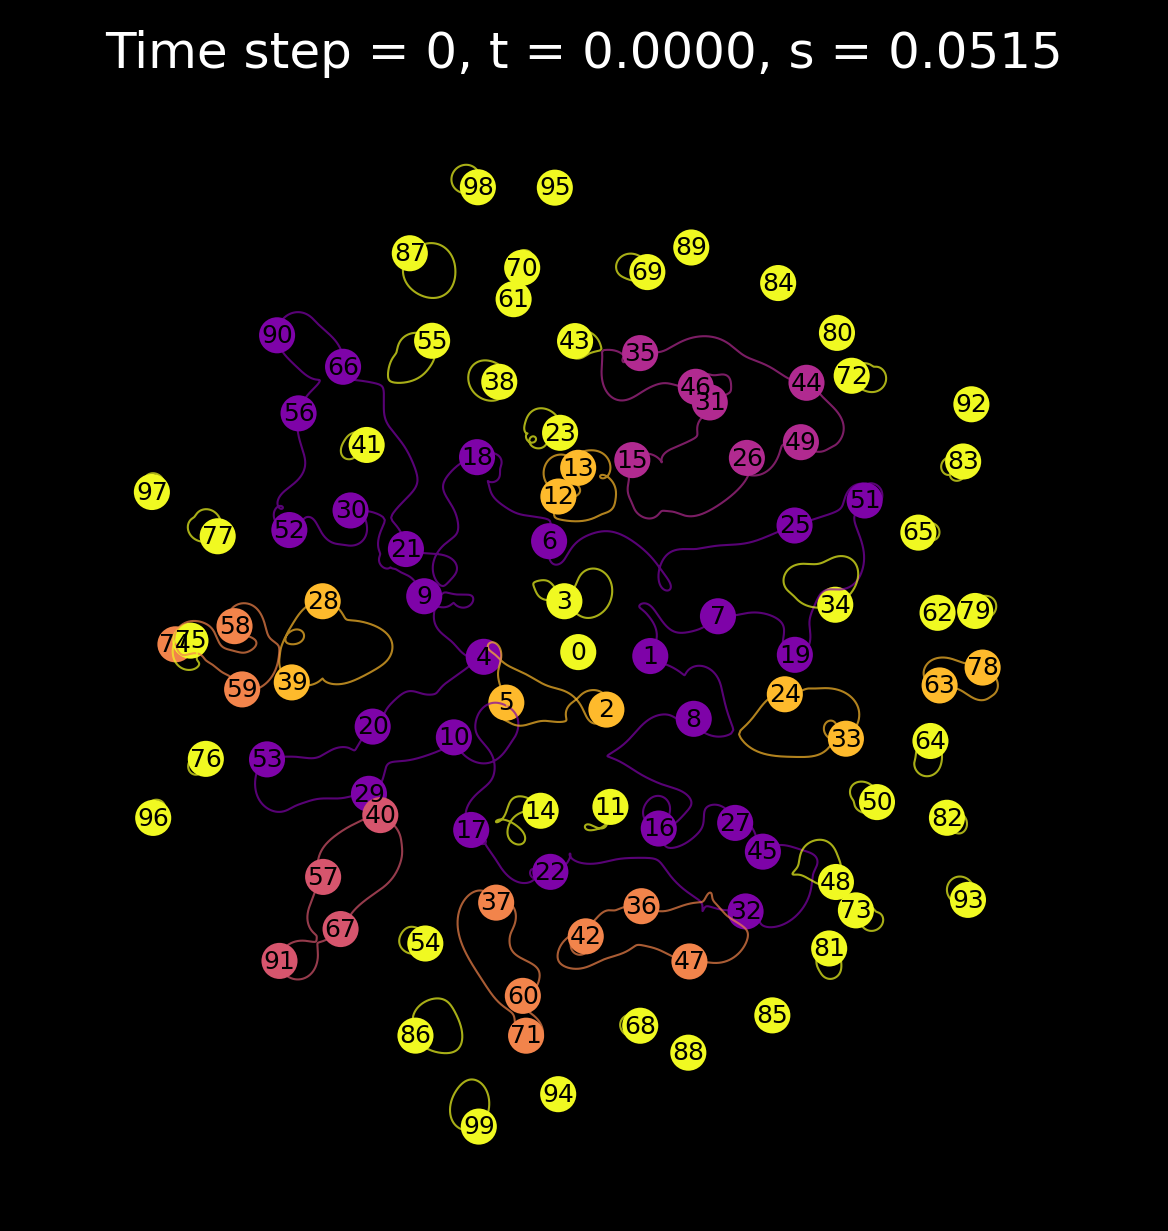
\includegraphics[width=\textwidth]{/home/charli/Math/eigenvalueTracking/animatedGinibre/N100s00515.png}
		\end{minipage}
	\end{figure}
	
	The corresponding permutations $\sigma(s_0)$, $\sigma(s_1)$, $\sigma(s_2)$, $\sigma(s_3)$ 
	all present small differences. 
	These are witness to \emph{eigenvalue collisions} 
	at some values $(s,t)$, $s \in (s_0, s_3)$.

	The collissions explain the permutation discrepancies in the following way: 
	if the eigenvalues $i$ and $j$ collided, 
	and they were originally pointing to $k$ and $l$, they will point after the collision 
	to $l$ and $k$ instead.
	
	The eigenvalues keep their initial tracks, 
	but switch paths after the value of $t$ where the collision occurred. 

	In the figure, there is a collision of the singleton $[58]$ and $59$, from the cycle $[59, 74]$ 
	between $s_0$ and $s_1$ 
	that makes produces the cycle [58, 59, 74] in the next frames.

	The next permutation configuration $\sigma(s_2)$ is explained by two collisions: 

	One collision ($27$ vs $36$) splits the 6-cycle $[32, 45, 27, 47, 42, 36]$ into two cycles 
	$[32, 45, 27], [47, 42, 36]$.

	The second collision $27$ vs $22$ (or the first, we are not sure of the order of the collisions 
	at the current refinement) joins the cycle $[47, 42, 36]$ with the large purple cycle.

	Finally, the last permutation is explained by two collisions: 
	One involving $91$ and $67$
	which joins the singleton [91] 
	from the cycle $[67, 57, 40]$, 
	to produce the 4-cycle $[67, 91, 57, 40]$

	The second is crash involving $21$ and $30$ which results in incorporating the 5-cycle ok $30$ 
	to the big purple cycle.

	Thus, we use these permutation discrepancies to detect eigenvalue collisions. 
	From computations for small $N$ we conjecture that there are exactly $N(N+1)$ 
	collisions as $s$ goes from $0$ to $1$. 

	We report some first statistics about these processes and their collisions.

	There is an interesting aspect about counting collisions: if a collision occurs 
	between two eigenvalues which are both not currently singletons, 
	then it is ambiguous to simply report that a given pair of eigenvalues crashed.
	
	The pairs of eigenvalues that acually crash depends on how we reach $R(s_0,t_0)$.
	Did we go in a straight line from $(0,0)$ to $(s_0,0)$ and then rotated?, or were we allowed
	to rotate at intermediate values $s$, $0 < s < s_0$?

	We include a simple package for these computations and visualizations. 
	
	From the $t$-processes we may extract different types of eigenvalue collision data
	for visualtization and/or statistics.

\end{document}

\section{References}

- P. Zhong. (include reference...)

\end{document}